\documentclass[]{article}

\usepackage{graphicx}
\usepackage[margin=1.0in]{geometry}

%opening
\title{Emory University at TREC LiveQA}
\author{Denis Savenkov\\Emory University\\dsavenk@emory.edu}
\date{}

\begin{document}

\maketitle

\begin{abstract}
This paper describes a question answering system built by a team from Emory University to participate in LiveQA TREC shared task.
Our system extracts candidates from answers to similar previously posted questions as well as from documents retrieved using web search API.
The candidates are ranked using single model, trained on question-answer (QnA) pairs from Yahoo! Answers WebScope dataset\footnote{https://webscope.sandbox.yahoo.com/catalog.php?datatype=l}.
The features used for ranking contains statistics over the candidate answer text, pairs of terms and their matches between question and answer texts and score from an LSTM neural network model, which is also trained on existing QnA pairs.

\end{abstract}

\section{Introduction}
Over the years of question answering research the focus was mainly around factoid questions, which constitute only a part of user information needs.
Community question answering (CQA) websites such as Yahoo! Answers\footnote{http://answers.yahoo.com/} contain millions of questions and answers posted by real users.
These questions are diverse and except factoid include opinion, advice, polls and many other types of questions. 
LiveQA TREC\footnote{http://trec-liveqa.org/} shared task requires a system to answer questions that have been posted to Yahoo! Answers and haven't been answered yet. 
The goal of the task is very interesting, promising and hopefully will lead to development of new systems moving the state-of-the-art in question answering further.

This was my first attempt to participate in TREC and due to time constraints I was able to implement a simple baseline system, which is based on a learning to rank model, trained on existing collection of QnA pairs.
The machine learning system was trained with the objective to rank the ``best''\footnote{By ``best'' we mean the answer that was selected as the best answer to the given question.} answer higher than answers to retrieved similar questions.
The system doesn't use any additional linguistic or other resources and do not try to classify questions into different types.
The goal was to see how well a general purpose system with simple feature can do on questions of various types.

\section{Approach}

The architecture of our system is presented on Figure \ref{figure:qa_model}.

\begin{figure}
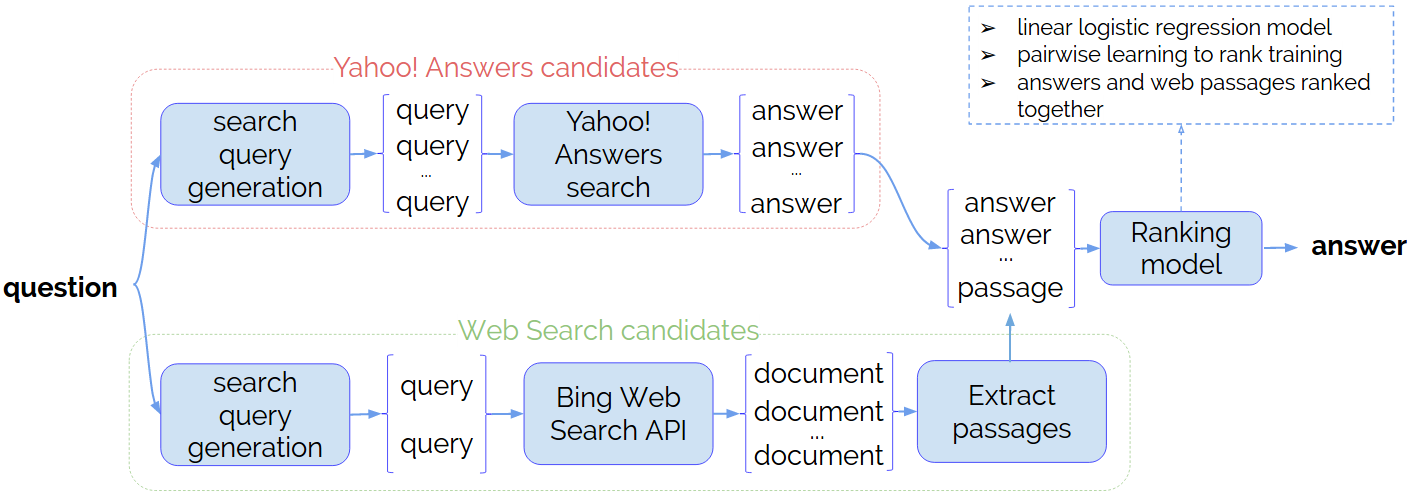
\includegraphics[width=450px]{img/qa_model}
\caption{Architecture of our question answering system}
\label{figure:qa_model}
\end{figure}


First, we attempt to get all the categories of the posted question from Yahoo!Answers website. I actually don't know if this is successful, the question might not be on the website yet. The reason for this step is that in the input we only get one category from the tree. I didn't have the tree myself, therefore I attempted to get the path from Yahoo!Answers.

Then we get the candidate answers from two sources independently: Yahoo!Answers similar questions search and Bing Web Search API.
For each of the sources we have separate query formulators.
From Yahoo! Answers we retrieve top 10 similar questions (for each query), for Web Search we retrieve top 5 documents.

For Yahoo! Answers we have many different query formulators:
\begin{itemize}
\item title + body
\item title
\item title + body without stopwords
\item title without stopwords
\item title + category name and without stopwords
\item title + body + category name without stopwords
\item top 5 tf-idf (based on Yahoo!Answers WebScope dataset) terms from the title
\item top 5 tf-idf (based on Yahoo!Answers WebScope dataset) terms from the title and body
\end{itemize}

For Web Search we only use the first two\footnote{we can cite AskMSR+, which showed that search already does a lot}.

For each retrieved web document we generate a set of candidate answers. We take snippet as candidate and also we generate fragments from contiguous sentences until the maximum length is reached (we only keep those that have non-zero term overlap with the question text).

Then for each candidate we generate a set of features and rank them with a linear ML model.

\begin{table}[t]
\label{table:features}
\caption{Features used to rank candidate answers}
\begin{tabular}{|c|p{10cm}|}
\hline
Feature name & Description \\
\hline
\hline
q-a lemma pairs & Concatenation of lemmas from question and answer texts\\
BM25 & BM25 scores of the candidate answer computed for the question title, body and concatenation of both. Collection statistics is taken from WebScope dataset of QnA pairs. \\
term matches & Outputs lemmas of terms matched in the question and answer text as well as percent and the total number of matched terms, POS tags of matched terms, length of the maximum span of matched terms\\
npmi & average, maximum and minimum normalized PMI scores between question and answer terms. NPMI scores are computed based on the WebScope collection of QnA pairs.\\
category match & boolean feature which is one if category of retrieved Yahoo! Answers QnA pair matches one asked\\
page title & Matches between question lemmas and lemmas of the retrieved page title. For Yahoo! Answers question text is used as the title.\\
answer stats & Statistics of the answer text, such as length in sentences in tokens, etc.\\
LSTM model & score returned for QnA pair by an LSTM model trained to predict the correct question-best answer pair\\
\hline
\end{tabular}
\end{table}

\section{Model Training}

\subsection{Logistic regression model}
To train the model I used WebScope dataset of QnA pairs from Yahoo. I built a search index with Apache Lucene and trained a linear ranking model. I took question + best selected answer and also retrieved answers to 10 most similar questions (by question title only) using Lucene BM25 retrieval model. Then I constructed training instances as pairwise feature differences for pairs of correct-retrieved answers. An instance is positive if we subtract features of the incorrect answer from features of the correct one. And instance is incorrect otherwise. We take all pairs. 
We train L2-regularized logistic regression.

\subsection{LSTM model}
LSTM model was also trained on WebScope dataset and in a similar way.
More specifically for each question from the dataset we use question title to retrieve similar questions using Lucene and then output 11 instances: one correct for question-best answer pair and then 10 question-retrieved answer. LSTM model (Figure \ref{figure:lstm_model}) is trained to classify correct QnA pairs.
Tokens of questions and answers are restricted to be at most 100 tokens. Then question and answer text are split using a sentinel separator token.
To make a binary prediction we used hidden state of the LSTM model after the whole QnA sequence is processed.

\begin{figure}
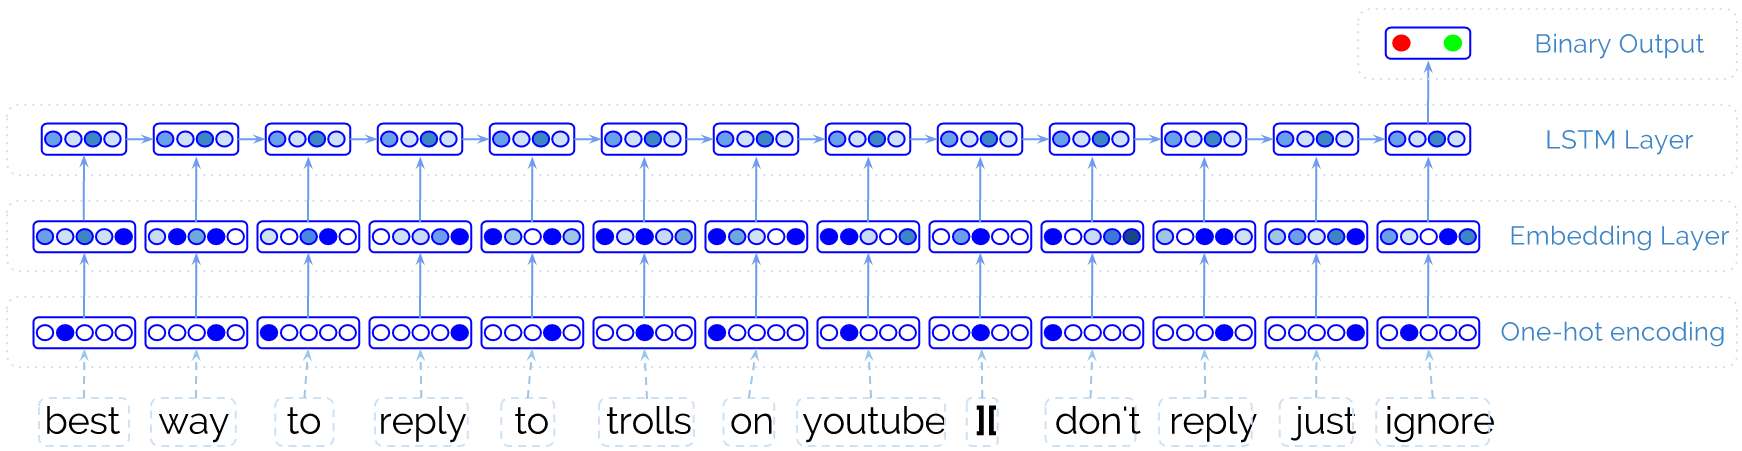
\includegraphics[width=450px]{img/qa_lstm}
\caption{LSTM model for predicting the correct answer}
\label{figure:lstm_model}
\end{figure}

We train the model using Adam stochastic gradient descent method \cite{kingma2014adam} with mini batches of size 200 instances for 100 epochs.

Parameters of the LSTM model:
\begin{itemize}
\item Embedding dimension 128
\item Hidden state size 128
\item Batch size 200
\item Epochs 100
\item Vocabulary size 1M
\end{itemize}

The model was implemented using Keras\footnote{http://keras.io/} library.

\section{Results}

Table \ref{table:liveqa-results} gives the results of Emory run and average scores for all runs.

\begin{table}
\caption{Results of the LiveQA evaluation}
\label{table:liveqa-results}
\begin{tabular}{|p{1.2cm}|p{1.2cm}|p{1.2cm}|p{1.2cm}|p{1.2cm}|p{1.2cm}|p{1.2cm}|p{1.2cm}|p{1.2cm}|}
\hline
name & avg score (0-3) & succ@1+ & succ@2+ & succ@3+ & succ@4+ & prec@2+ &
 prec@3+ & prec@4+ \\
 \hline
Emory run & 0.605 & 0.812 & 0.332 & 0.190 & 0.086 & 0.408 & 0.233 & 0.106\\
\hline
Average of all runs & 0.465 & 0.925 & 0.262 & 0.146 & 0.060 & 0.284 & 0.159 & 0.065\\
\hline
\end{tabular}
\end{table}

General statistics:
Overall, 1087 questions were judged and scored using 4-level scale:\\
4: Excellent -- a significant amount of useful information, fully answers the question\\
3: Good – partially answers the question\\
2: Fair -- marginally useful information\\
1: Bad – contains no useful information for the question\\
-2: the answer is unreadable  (only 15 answers from all runs were judged as unreadable)

The performance measures are:\\
avg-score(0-3) - average score over all queries (transferring 1-4 level scores to 0-3, hence comparing 1-level score with no-answer score, also considering -2-level score as 0)\\
succ@i+ - number of questions with i+ score (i=1..4) divided by number of all questions\\
prec@i+ - number of questions with i+ score (i=2..4) divided by number of answered only questions\\

\section{Related Work}

\section{Conclusion}

\bibliography{bibliography.bib}

\end{document}
